\section{实验原理}

传统的人工神经网络(ANN)基于电子器件模拟神经系统的结构,建立神经网络各层神经元之间的联系,然而,电子器件的速度和功耗等方面的限制,使得传统的人工神经网络在训练和推理过程中存在一定的局限性。最初的神经网络基于CPU训练,但无法满足深度网络中大量浮点和并行运算的要求;之后,基于GPU的神经网络训练方法得到了广泛应用,然而电信号的能耗和物理限制仍然是一个问题。因此,寻找一种新的神经网络训练和推理方法是非常重要的。

作为替代,将光作为媒介是一个可行的方法,光速高达每秒30万公里,且并行性高、抗干扰性强,在信息传输和光计算方面具有巨大优势。光学神经网络(ONN)天然具有并行性和高速性,因此在训练和推理过程中具有很大的优势。光学神经网络的基本原理是利用光学器件的非线性特性,将神经网络的激活函数和权重参数映射到光学器件的物理参数上,通过光学器件的非线性特性来实现神经网络的训练和推理过程。训练完成之后,整个结构就能以光速进行光信号计算,而无需额外的能量输入。

本章节将介绍光学神经网络的基本原理,包括傅立叶变换、非线性光学器件、光学神经网络等内容。

\subsection{傅立叶变换}

时域和频域是信号处理中常用的两种表示方法,时域表示信号随时间的变化,频域表示信号的频率特性。傅立叶变换是一种将信号从时域转换到频域的数学工具,可以更好地理解信号的频率特性。而对于二维图像来说,傅立叶变换可以将图像从空域转换到频域,从而可以更好地理解图像的频率特性。

% pics/time_domain_vs_frequency_domain.png / space_domain_vs_frequency_domain.png 子图左右排列,基于subfloat
\begin{figure}[H]
    \centering
    \subfloat[时域和频域]{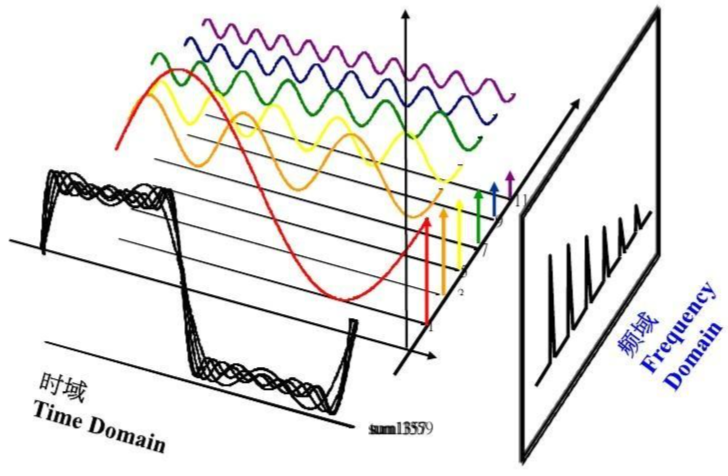
\includegraphics[width=0.45\textwidth]{pics/time_domain_vs_frequency_domain.png}}
    \subfloat[空域和频域]{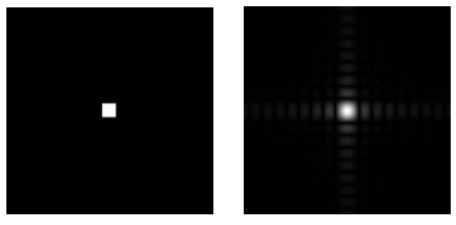
\includegraphics[width=0.45\textwidth]{pics/space_domain_vs_frequency_domain.png}}
    \caption{时域和频域、空域和频域}
    \label{fig:time_domain_and_space_domain}
\end{figure}

如图\ref{fig:time_domain_and_space_domain}所示,时域信号可以通过傅立叶变换转换为频域信号,空间域图像也可以通过傅立叶变换转换为频域图像。对于一维信号来说,时域信号表示信号随时间的变化,频域信号则表示信号在不同频率上的分量;对于二维图像来说,空域图像表示图像的像素值,频域图中的每个像素表示图像在不同方向和频率上的分量。

傅立叶变换是一种信号处理中常用的数学工具,它可以将一个信号从时域转换到频域。具体来说,任意信号都可以表示为不同频率的正弦波的叠加,傅立叶变换可以将信号分解为不同频率的正弦波,从而可以更好地理解信号的频率特性。傅立叶变换可以表示为公式\ref{eq:fourier}:

\begin{equation}
    F(\omega) = \int_{-\infty}^{\infty} f(t) e^{-j\omega t} dt
    \label{eq:fourier}
\end{equation}

其中,$F(\omega)$是信号$f(t)$的傅立叶变换,$\omega$是频率,$j$是虚数单位。傅立叶变换可以将信号从时域转换到频域,从而可以更好地理解信号的频率特性。

对于图像来说,傅立叶变换同样可以将图像从空间域转换到频域。这是因为任意图像都可以看作是一个二维的信号,傅立叶变换同样可以将图像分解为各个不同方向和频率的正弦波,从而可以更好地理解图像的频率特性。二维图像的傅立叶变换可以表示为公式\ref{eq:fourier2d}:

\begin{equation}
    F(u, v) = \iint f(x, y) e^{-j2\pi(ux+vy)} dx dy
    \label{eq:fourier2d}
\end{equation}

其中,$F(u, v)$是图像$f(x, y)$的二维傅立叶变换,$u$和$v$是频率,$j$是虚数单位。二维傅立叶变换可以将图像从空域转换到频域,从而可以更好地理解图像的频率特性。

\subsection{非线性光学效应}

非线性光学效应是指光信号在非线性介质中传播时,光信号的强度、相位等参数会发生非线性变化。当光通过晶体进行传播时,会引起晶体的电极化。对于某些材料来说,在光强不太大时,晶体的电极化强度与光频电场之间呈线性关系,这种非线性关系可以被忽略;但是,当光强很大时,例如激光通过晶体传播时,电极化强度与光频电场之间的非线性关系变得显著。

1961年,美国科学家Franken首次发现了晶体的非线性光学效应,他将红宝石产生的激光入射到石英晶体上,发现射出的光束除了红宝石的693.4nm波长外,还有347.2nm的波长。这种现象被称为二次谐波产生,是晶体的非线性光学效应的一个典型例子。之后,人们发现了更多的非线性光学材料,如BBO、LBO等,这些材料可以实现更多种类的非线性光学效应。

% pics/shg.png
\begin{figure}[H]
    \centering
    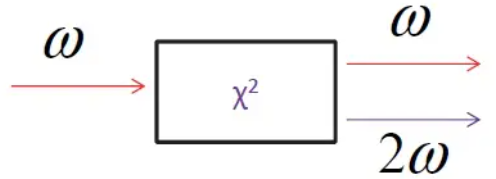
\includegraphics[width=0.4\textwidth]{pics/shg.png}
    \caption{二次谐波产生}
    \label{fig:shg}
\end{figure}

极化现象是非线性光学效应的基础,当光激发材料时,材料中的电子会发生位移,从而产生电偶极矩。材料在光激发时会发生极化,极化强度与光频电场之间的关系可以表示为公式\ref{eq:polarization}:

\begin{equation}
    P(t) = \varepsilon_0 \chi^{(1)} E(t) + \varepsilon_0 \chi^{(2)} E^2(t) + \varepsilon_0 \chi^{(3)} E^3(t) + \cdots = P^L + P^{NL}
    \label{eq:polarization}
\end{equation}

其中,$P(t)$是极化强度,$\varepsilon_0$是真空介电常数,$\chi^{(1)}$、$\chi^{(2)}$、$\chi^{(3)}$等是非线性极化系数,$E(t)$是光频电场,$P^L$是线性极化,$P^{NL}$是非线性极化。当光强不太大时,非线性极化可以忽略,此时极化强度与光频电场之间呈线性关系;但是,当光强很大时,非线性极化变得显著,此时极化强度与光频电场之间呈非线性关系。

\subsection{光学神经网络}

光学神经网络(ONN)是一种基于光学器件的神经网络,利用光学器件的非线性特性来实现神经网络的训练和推理过程。光学神经网络的基本原理是将神经网络的激活函数和权重参数映射到光学器件的物理参数上,通过光学器件的非线性特性来实现神经网络的训练和推理过程。

光学神经网络可以在空间域中进行计算,即将输入信号通过光学器件进行传播,然后通过光学器件的非线性特性来实现神经网络的训练和推理过程。传统的电子神经网络中的每一层输出通过电子器件计算:

\begin{equation}
    X^{l+1}=F^l(W^l\cdot X^l+B^l)
\end{equation}

其中$W^l,B^l$是可学习参数。而全光深度衍射神经网络(D2NN)是一种基于光学器件的神经网络,该网络由一个输入层、若干个中间衍射层和一个输出层组成,网络的输入是相干光,并且在每个衍射层都会发生衍射产生二次波。具体来说,通过控制光相位和幅值,可以改变衍射层的投射和反射系数,从而控制衍射层的权重参数进行计算:

\begin{equation}
    Y^{l+1}=F^l(W^l\cdot X^l+B^l), Y^{l}=X^{l}{e^j}^{\psi^l}
\end{equation}

其中$\psi^l$是相位参数。全光深度衍射神经网络的结构如图\ref{fig:d2nn}所示,D2NN通过对相干光进行衍射,控制光的相位和幅值,最后通过将光信号划分为多个区域,根据最大值光信号的位置来判断输出结果。对于模型训练,可以通过计算机模拟光传播的过程,然后通过梯度下降等方法来更新光学器件的参数。

% pics/d2nn.png
\begin{figure}[H]
    \centering
    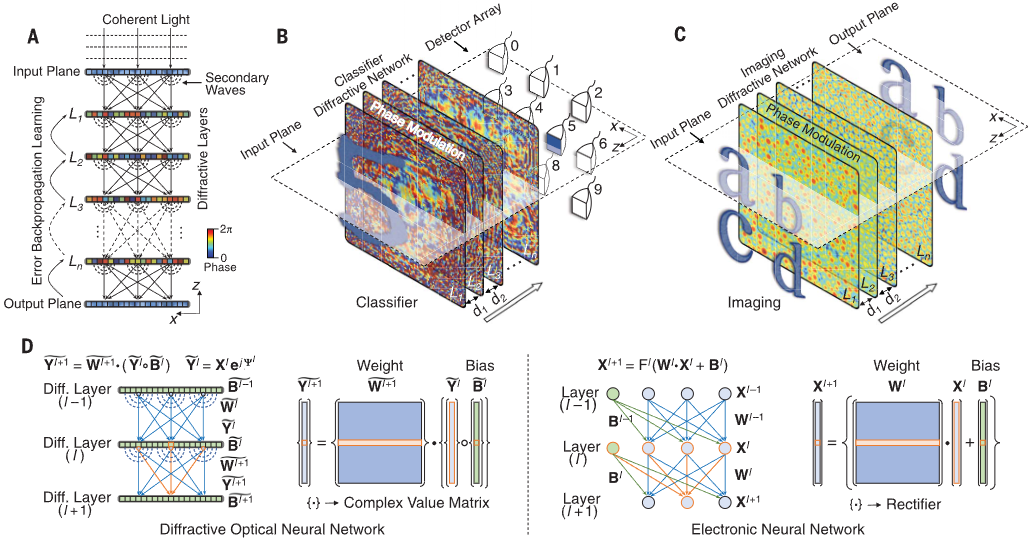
\includegraphics[width=0.9\textwidth]{pics/d2nn.png}
    \caption{全光深度衍射神经网络}
    \label{fig:d2nn}
\end{figure}

此外,光学神经网络还可以在频域中进行计算,即将输入信号通过傅立叶变换转换到频域,然后通过光学器件的非线性特性来实现神经网络的训练和推理过程。傅立叶衍射网络(F-D2NN)同样由一个输入层、若干个中间衍射层和一个输出层组成,不同的是,F-D2NN的输入是经过傅立叶变换的信号,中间衍射层加入了非线性器件,而输出层则是通过傅立叶逆变换将信号转换回空间域。

傅立叶变换域逆变换是通过2f系统实现的,2f系统是一种光学系统,可以将输入信号通过透镜成像到傅立叶平面,然后通过另一个透镜将信号成像到输出平面。输入光信号首先通过透镜成像到傅立叶平面,然后通过D2NN网络进行计算,之后通过非线性单元,最后通过透镜将信号成像到输出平面。这一过程可以表示为:

\begin{equation}
    \hat{U}_0=FU_0,\hat{U_1}=\hat{M}\hat{U}_0,\hat{U}_2=\phi(\hat{U}_1),O=|F\hat{U}_2|^2
    \label{eq:fd2nn}
\end{equation}

其中,$U_0$是输入信号,$F$是傅立叶变换,$\hat{M}$是D2NN网络,$\phi$是非线性单元,$O$是输出信号。F-D2NN的结构如图\ref{fig:fd2nn}所示,经过变换,光信号转换为输出信号,然后可以用于图像分类、显著目标检测等任务。

% pics/fd2nn.png
\begin{figure}[H]
    \centering
    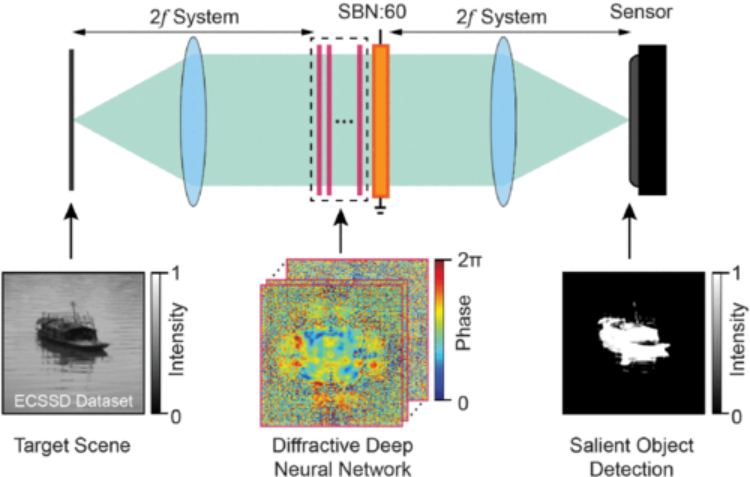
\includegraphics[width=0.7\textwidth]{pics/fd2nn.png}
    \caption{傅立叶衍射网络}
    \label{fig:fd2nn}
\end{figure}